%!TEX root = ../dissertation.tex
\begin{savequote}[75mm]
Ugliness is in a way superior to beauty because it lasts.
\qauthor{Serge Gainsbourg}
\end{savequote}
%%%%%%%%%%%%%%
\chapter{Data and Simulation}
%\subsection{Dataset}

\paragraph{}
The studies presented in this note are based on the 2015 and 2016 dataset at $\sqrt{s}=13$~TeV recorded by the ATLAS experiment~\cite{detPaper}. Jet triggers were used to select the data (details below). The analysis also ran over the 2015 and the 2016 debug stream, in which no events that pass the full event selection were found. The 2015 dataset corresponds to a total integrated luminosity of 3.2\, fb$^{-1}$, and the 2016 dataset corresponds to a total integrated luminosity of 32.9\, fb$^{-1}$. The total luminosity is 36.1\, fb$^{-1}$.

\paragraph{}
The analysis is based on EXOT8 derivations of the xAOD, the contents of which can be found at \href{https://svnweb.cern.ch/trac/atlasoff/browser/PhysicsAnalysis/DerivationFramework/DerivationFrameworkExotics/trunk/share/EXOT8.py}{DerivationFrameworkExotics/EXOT8}. The 20.7.8.7 derivation cache was used in the analysis, which corresponds to \texttt{DerivationFrameworkExotics-00-03-86} and $p$-tags \texttt{p2950}. The boosted slimming keeps events with at least two large-$R$ jets with \pt~$>$200 GeV. 
%In the derivationt here is another cut requiring there are at least two trackjets with MV2c10 score greater than -10. Because there is no pT cut, this requirement is almost always passed--events doesn't pass this hints the large-R jet has one and only one tracking activities, which is also probably a good idea to keep it out. However, this should be modified in the future.

\paragraph{}
The studies presented currently in the main context of this note are extended to incorporate 2016 data. In this note, the reconstruction of both the 2015 and 2016 datasets are performed using software release 20.7. Simulated data samples from the mc15c campaign are be used, corresponding to $p$-tags \texttt{p2952-p2949}.
% to look up derivation tag info:
% > grep Exotics /cvmfs/atlas.cern.ch/repo/sw/software/x86_64-slc6-gcc48-opt/20.1.8/AtlasDerivation/20.1.8.5/AtlasDerivationRelease/cmt/requirements
% https://twiki.cern.ch/twiki/bin/viewauth/AtlasProtected/DerivationProductionTeam#Info_on_AtlasDerivation_caches_a

\paragraph{}
The 2015 data sets from release 20.7 that are currently used in this analysis are:
\noindent
\\
{\scriptsize
\verb|data15_13TeV.periodD.physics_Main.PhysCont.DAOD_EXOT8.grp15_v01_p2950|\\
\verb|data15_13TeV.periodE.physics_Main.PhysCont.DAOD_EXOT8.grp15_v01_p2950|\\
\verb|data15_13TeV.periodF.physics_Main.PhysCont.DAOD_EXOT8.grp15_v01_p2950|\\
\verb|data15_13TeV.periodG.physics_Main.PhysCont.DAOD_EXOT8.grp15_v01_p2950|\\
\verb|data15_13TeV.periodH.physics_Main.PhysCont.DAOD_EXOT8.grp15_v01_p2950|\\
\verb|data15_13TeV.periodJ.physics_Main.PhysCont.DAOD_EXOT8.grp15_v01_p2950|
}

\paragraph{}
The current 2016 data sets are:
\noindent
\\
{\scriptsize
\verb|data16_13TeV.periodA.physics_Main.PhysCont.DAOD_EXOT8.grp16_v01_p2950|\\
\verb|data16_13TeV.periodB.physics_Main.PhysCont.DAOD_EXOT8.grp16_v01_p2950|\\
\verb|data16_13TeV.periodC.physics_Main.PhysCont.DAOD_EXOT8.grp16_v01_p2950|\\
\verb|data16_13TeV.periodD.physics_Main.PhysCont.DAOD_EXOT8.grp16_v01_p2950|\\
\verb|data16_13TeV.periodE.physics_Main.PhysCont.DAOD_EXOT8.grp16_v01_p2950|\\
\verb|data16_13TeV.periodF.physics_Main.PhysCont.DAOD_EXOT8.grp16_v01_p2950|\\
\verb|data16_13TeV.periodG.physics_Main.PhysCont.DAOD_EXOT8.grp16_v01_p2950|\\
\verb|data16_13TeV.periodI.physics_Main.PhysCont.DAOD_EXOT8.grp16_v01_p2950|\\
\verb|data16_13TeV.periodK.physics_Main.PhysCont.DAOD_EXOT8.grp16_v01_p2950|\\
\verb|data16_13TeV.periodL.physics_Main.PhysCont.DAOD_EXOT8.grp16_v01_p2950|
}


\clearpage
\subsection{Simulated signal and background samples}
\paragraph{}
All MC samples used in this analysis are produced with full simulation, with additional \pileup interactions in each simulated event 
modeled by adding multiple soft $pp$ collisions
generated by \Pythia~8.165~\cite{pythia8} with the MSTW2008 LO PDF and AU2 tune~\cite{MC12AU2}.  After event generation and the addition of \pileup, 
the response of the ATLAS detector to particles
passing through the detector elements is simulated with the GEANT4 toolkit~\cite{Geant4,simulation}
and events are reconstructed using the same software used to reconstruct events in data.
%Simulation events are further corrected to reproduce the amount of pileup produced in the data, using the standard ATLAS pileup reweighting tool~\cite{pileuptwiki}.

\subsubsection{Signal MC production}
%A non-resonant SM signal sample has been generated using aMC@NLO. These \ggtofourb events are generated at NLO, using the exact form factors for the top loop taken from HPAIR~\cite{PhysRevD.58.115012,Plehn199646}. The sample is:
%\begin{Verbatim}[fontsize=\scriptsize]
%mc15_13TeV.342619.aMcAtNloHerwigppEvtGen_UEEE5_CTEQ6L1_CT10ME_hh_4b.merge.DAOD_EXOT8.e4419_s2608_r6869_r6282_p2454.
%\end{Verbatim}

%The gluon-fusion production cross-section used is evaluated at NNLO+NNLL in QCD \cite{LHCHXSWGHH}: $\sigma(pp\rightarrow hh\rightarrow b\bar{b}b\bar{b})~=~12.7\pm1.6$\,fb, where the uncertainty term includes the effects of uncertainties in the renormalization and factorization scale, PDFs, $\alpha_S$, effects of finite $m_t$ in loops and $Br\left(H\rightarrow b\bar{b}\right)$.
%, summed with the NLO predictions for vector-boson-fusion, top-pair-associated and vector-boson-associated production from Ref.~\cite{1401.7340}. The resulting cross-section is $\sigma(pp\rightarrow hh\rightarrow b\bar{b}b\bar{b}) = 3.6\pm0.5$\,fb, where the uncertainty term includes the effects of uncertainties in the renormalization and factorization scale, PDFs, $\alpha_S$ and $Br\left(H\rightarrow b\bar{b}\right)$.

\paragraph{}
Two benchmark resonant signal models are considered: a spin-2 graviton within a Bulk Randall-Sundrum Kaluza-Klein model and a spin-0 heavy neutral Higgs boson within a 2HDM model. 

\paragraph{}
The Bulk RS KK graviton signal samples have been generated for 20 mass points from 300 to 3000\,GeV using the \Madgraph generator\cite{MG5aMCatNLO} with the NNPDF2.3 LO PDF~\cite{Ball:2012cx} and the A14 tune \cite{ATL-PHYS-PUB-2014-021}, and hadronic showers are produced in \Pythia8.  For all signal samples, the Higgs mass has been set to 125.0 GeV. The cross-section times branching ratio values are reported in Tables \ref{tab:signal_c10_xsec} and \ref{tab:signal_c20_xsec}, setting $c \equiv k/\bar{M}_P$ to 1.0 and 2.0, respectively.  The names of signal datasets are listed in Appendix~\ref{app:signal-samples}. Concerning the level of freedom in his model, Kaustubh Agashe~\cite{Agashe} suggested that $c$ cannot be increased much beyond two.

\paragraph{}
For signal kinematic distributions, see Appendix~\ref{app:signal-dist}.
%\Figref{signal-samples} shows the RSG mass for the simulated signal points.  The larger intrinisc width of the RS graviton resonance for $c=2$ can be seen, as the width increases as the square of the coupling (see \Eref{RSwidth}). The cross-section times branching ratio values for the 2HDM samples are reported in Table \ref{tab:signal_2hdm_xsec}.

\begin{table}[htbp]
\begin{center}
\begin{tabular}{c | c | c | c | c | c}
\hline
   DSID  &  $m_{G_{KK}}$ (GeV)   &  $\Gamma_{G_{KK}}$  (GeV) &   $\sigma \times$ BR($G_{KK}\to hh$) (fb) &  BR($G_{KK}\to hh$) & $N_{events}$ \\
\hline
 301488  & 300 & 8.365 & 1319.9 $\pm$ 1.0 & 0.90 & 79000 \\
301490 & 500 &18.43 & 892.4 $\pm$ 0.6 & 6.43 & 93400\\ 
301491 & 600 & 26.08 & 410.4 $\pm$ 0.3 & 6.95 & 99000\\ 
301492 & 700 & 33.65 & 201.48 $\pm$ 0.15 & 7.19 & 54000\\ 
301493 & 800 & 41.06 & 105.49 $\pm$ 0.07 & 7.33 & 70000\\ 
301494 & 900 & 48.30 & 58.35 $\pm$ 0.04 & 7.41 & 85000\\ 
301495 & 1000 & 55.40 & 33.68 $\pm$ 0.02 & 7.47& 100000\\ 
301496 & 1100 & 62.38 & 20.23 $\pm$ 0.01 & 7.51 & 99000\\
301497 & 1200 & 69.27 & 12.54 $\pm$ 0.01 & 7.54 & 99000\\
301498 & 1300 & 76.09 & 7.979 $\pm$ 0.005 & 7.56 & 19000\\
301499 & 1400 & 82.84 & 5.201 $\pm$ 0.004 & 7.58 & 98600 \\
301500 & 1500 & 89.54 & 3.450 $\pm$ 0.002 & 7.59 & 99000\\
301501 & 1600 & 96.20 & 2.336 $\pm$ 0.002 & 7.60 & 99000\\
301502 & 1800 & 109.4 & 1.116 $\pm$ 0.001 & 7.62 & 15000\\
301503 & 2000 & 122.5 & $0.5559 \pm 3\times10^{-4}$ & 7.63 & 88800\\
301504 & 2250 & 138.8 & $0.2486 \pm 2\times10^{-4}$ & 7.64 & 99000\\
301505 & 2500 & 155.0 & $0.1158 \pm 1\times10^{-4}$ & 7.65 & 60000\\
301506 & 2750 & 171.1 & $0.05585 \pm 4\times10^{-5}$ & 7.66 & 58600\\
301507 & 3000 & 187.2 & $0.02772 \pm 2\times10^{-5}$ & 7.66 & 78000\\
\hline
\end{tabular}
\caption{Cross-section times branching ratio for RS graviton samples with $c \equiv k/\bar{M}_P = 1.0$ 
as a function of the graviton mass.}
\label{tab:signal_c10_xsec}
\end{center}
\end{table}

\begin{table}[htbp]
\begin{center}
\begin{tabular}{c | c | c | c | c | c}
\hline
   DSID  &  $m_{G_{KK}}$ (GeV)   &  $\Gamma_{G_{KK}}$  (GeV) &   $\sigma \times$ BR($G_{KK}\to hh$) (fb) &  BR($G_{KK}\to hh$) & $N_{events}$ \\
\hline
301508 & 300 & 33.46 & 9997 $\pm$ 11 & 0.90 & 90000\\
301509 & 400 & 45.22 & 8560 $\pm$ 7 & 4.99 & 60000\\
301510 & 500 & 73.74 & 3755 $\pm$ 3 & 6.43 & 100000\\
301511 & 600 & 104.3 & 1657 $\pm$ 1 & 6.95 & 98800\\
301512 & 700 & 134.6 & 789.9 $\pm$ 0.6 & 7.19 & 99000\\
301513 & 800 & 164.2 & 404.3 $\pm$ 0.3 & 7.33 & 99000\\
301514 & 900 & 193.2 & 219.3 $\pm$ 0.2 & 7.41 & 100000\\
301515 & 1000 & 221.6 & 125.1 $\pm$ 0.1 & 7.47 & 100000\\
301516 & 1100 & 249.5 & 74.19 $\pm$ 0.05 & 7.51 & 58600\\
301517 & 1200 & 277.1 & 45.48 $\pm$ 0.003 & 7.54 & 74000\\
301518 & 1300 & 304.4 & 28.72 $\pm$ 0.02 & 7.56 & 100000\\
301519 & 1400 & 331.4 & 18.55 $\pm$ 0.001 & 7.58 & 73800\\
301520 & 1500 & 358.2 & 12.27 $\pm$ 0.001 & 7.59 & 99000\\
301521 & 1600 & 384.8 & 8.254 $\pm$ 0.005 & 7.60 & 100000\\
301522 & 1800 & 437.7 & 3.913 $\pm$ 0.003 & 7.62 & 93400\\
301523 & 2000 & 490.1 & 1.951 $\pm$ 0.001 & 7.63 & 60000\\
301524 & 2250 & 555.2 & 0.8703 $\pm$ 0.0006 & 7.64 & 100000\\
301525 & 2500 & 620.0 & 0.4070 $\pm$ 0.0003 & 7.65 & 84000\\
\hline
\end{tabular}
\caption{Cross-section times branching ratio for RS graviton samples with $c \equiv k/\bar{M}_P = 2.0$ 
as a function of the graviton mass.}
\label{tab:signal_c20_xsec}
\end{center}
\end{table}

\paragraph{}
The heavy Higgs boson samples have been generated for the same 20 mass points from 300 to 3000\,GeV using the \Madgraph generator\cite{MG5aMCatNLO} with the 
CT10 PDF set. Hadronic showers are produced in \herwigpp using CTEQ6L1 and the UEEE5 event tune. 
For all signal samples, the Higgs boson mass has been set to 125.0 GeV. The width of the heavy Higgs boson, $\Gamma_H$, has been set to 1 GeV. This is because the width is dependent on 2HDM parameters. In Run-1, limits were set based on parameterised signal mass distributions with a representative range of widths.
\paragraph{}
To illustrate the properties of the $H$, a phase-space point \cba = 0.2, \tanb = 1 has been chosen within a Type-2 2HDM. The heavy Higgs boson partners' ($H, A, H^{\pm}$) masses are set such that $m_H = m_A = m_{H^{\pm}}$. The potential parameter that mixes the two Higgs doublets, $m_{12}$, is fixed such that $m_{12}^2 = m_A^2\tanb/(1+\tan^2\beta)$. This phase-space point has not been excluded by coupling measurements of the observed SM-like Higgs boson and is on the cusp of the observed 95\% C.L. exclusion of the Run 1 \Htohhb analysis. The relevant 2HDM properties are obtained from the HBSM group's ntuple for $\sqrt{s} = 13$\,TeV, version 1.6.3 \cite{HBSMNtuple}. They are reported in Table \ref{tab:signal_2hdm_xsec}.

\begin{table}[h]
\begin{center}
\begin{tabular}{c | c | c | c | c | c}\hline
DSID & $m_H$ (GeV) & $\Gamma_H$ (GeV) & $\sigma\times$Br($H\to hh \to b\bar{b}$) (pb) &  BR($H\to hh$) & $N_{\rm{events}}$\\\hline
343394 & 260 & 0.378 & 0.852 				& 0.489 &  -  \\
343395 & 300 & 0.961 & 0.925 				& 0.647 &  - \\
343396 & 400 & 5.84 & 0.522 				& 0.398 &  - \\
343397 & 500 & 15.2 & 0.211 				& 0.348 &  - \\
343398 & 600 & 26.0 & $9.96\times10^{-2}$ 	& 0.377 &  - \\
343399 & 700 & 38.9 &$ 5.02597\times10^{-2}$ & 0.418 &  - \\
343400 & 800 & 54.5 & $2.6561\times10^{-2}$ & 0.458 &  - \\
343401 & 900 & 73.2 & $1.45677\times10^{-2}$ & 0.494 &  - \\
343402 & 1000 & 95.6 & $8.24653\times10^{-3}$ & 0.525 &  - \\
343403 & 1100 & 122 & $4.79918\times10^{-3}$ & 0.552 &  - \\
343404 & 1200 & 154 & $2.86249\times10^{-3}$ & 0.575 &  - \\
343405 & 1300 & 190 & $1.74553\times10^{-3}$ & 0.594 &  - \\
343406 & 1400 & 232 & $1.08577\times10^{-3}$ & 0.610 &  - \\
343407 & 1500 & 280 & $6.87569\times10^{-4}$ & 0.624 &  - \\
\hline
\end{tabular}
\caption{Heavy Higgs boson properties for Type-2 2HDM with \cba = 0.2 and \tanb = 1. \BrHhh, \Brhbb and $\Gamma_H$ are parameter-dependent. The MC samples were generated with $\Gamma_H = 1$\,GeV.}
\label{tab:signal_2hdm_xsec}
\end{center}
\end{table}
 
%\begin{figure}[ht!]
%\begin{center}
%   %\includegraphics[angle=270, width=0.45\textwidth]{figures/truth_plots/masses_RSG_c10.pdf}
%   %\includegraphics[angle=270, width=0.45\textwidth]{figures/truth_plots/masses_RSG_c20.pdf}
%\caption{RSG signal mass points for $c=1.0$ (left) and $c=2.0$ (right).}
%\label{fig:signal-samples}
%\end{center}
%\end{figure}

\clearpage
\subsubsection{Background simulation}
\paragraph{}
While the dominant QCD multijet background (about 90\% of the total) was estimated in data, a \Pythia~\cite{pythia8} dijet sample was used to understand the physical processes contributing to this background and characteristics of the event selection. The usefulness of this background sample is limited by the generated number of events, given the high background rejection factors of the analysis selection. The dijet samples are listed below.
\\ \\
\noindent
{\scriptsize
\verb|mc15_13TeV.361020.Pythia8EvtGen_A14NNPDF23LO_jetjet_JZ0W.merge.DAOD_EXOT8.e3569_s2576_s2132_r7725_r7676_p2949|\\
\verb|mc15_13TeV.361021.Pythia8EvtGen_A14NNPDF23LO_jetjet_JZ1W.merge.DAOD_EXOT8.e3569_s2576_s2132_r7725_r7676_p2949|\\
\verb|mc15_13TeV.361022.Pythia8EvtGen_A14NNPDF23LO_jetjet_JZ2W.merge.DAOD_EXOT8.e3668_s2576_s2132_r7725_r7676_p2949|\\
\verb|mc15_13TeV.361023.Pythia8EvtGen_A14NNPDF23LO_jetjet_JZ3W.merge.DAOD_EXOT8.e3668_s2576_s2132_r7725_r7676_p2949|\\
\verb|mc15_13TeV.361024.Pythia8EvtGen_A14NNPDF23LO_jetjet_JZ4W.merge.DAOD_EXOT8.e3668_s2576_s2132_r7725_r7676_p2949|\\
\verb|mc15_13TeV.361025.Pythia8EvtGen_A14NNPDF23LO_jetjet_JZ5W.merge.DAOD_EXOT8.e3668_s2576_s2132_r7725_r7676_p2949|\\
\verb|mc15_13TeV.361026.Pythia8EvtGen_A14NNPDF23LO_jetjet_JZ6W.merge.DAOD_EXOT8.e3569_s2608_s2183_r7725_r7676_p2949|\\
\verb|mc15_13TeV.361027.Pythia8EvtGen_A14NNPDF23LO_jetjet_JZ7W.merge.DAOD_EXOT8.e3668_s2608_s2183_r7725_r7676_p2949|\\
\verb|mc15_13TeV.361028.Pythia8EvtGen_A14NNPDF23LO_jetjet_JZ8W.merge.DAOD_EXOT8.e3569_s2576_s2132_r7772_r7676_p2949|\\
\verb|mc15_13TeV.361029.Pythia8EvtGen_A14NNPDF23LO_jetjet_JZ9W.merge.DAOD_EXOT8.e3569_s2576_s2132_r7772_r7676_p2949|\\
\verb|mc15_13TeV.361030.Pythia8EvtGen_A14NNPDF23LO_jetjet_JZ10W.merge.DAOD_EXOT8.e3569_s2576_s2132_r7772_r7676_p2949|\\
\verb|mc15_13TeV.361031.Pythia8EvtGen_A14NNPDF23LO_jetjet_JZ11W.merge.DAOD_EXOT8.e3569_s2608_s2183_r7772_r7676_p2949|\\
\verb|mc15_13TeV.361032.Pythia8EvtGen_A14NNPDF23LO_jetjet_JZ12W.merge.DAOD_EXOT8.e3668_s2608_s2183_r7772_r7676_p2949|
}

%\Figref{pdgid-bg} demonstrates that the dominant multijet background is principally composed events arising from gluons (which then split to $b\bar{b}$), with less than 1 part per mille arising from light quarks or direct b-quark production.

%\begin{figure}[ht!]
%\begin{center}
%   %\includegraphics[angle=270, width=0.5\textwidth]{figures/truth_plots/dijet_pdgId_4b_boosted.png}
%\caption{PDG values of a multijet background as well as various RS graviton signal samples.  The QCD background is primarily composed
%of jets arising from gluons (PDG ID = 21).}
%\label{fig:pdgid-bg}
%\end{center}
%\end{figure}

\paragraph{}
The \ttbar\ background is modeled using large all-hadronic and non-all-hadronic decay mode samples that have both been generated with \Powheg~\cite{powheg} and showered with \Pythia~\cite{pythia8}. The top mass in both samples is set to 172.5 GeV. Samples inclusive in $m_{tt}$ are listed here:
\\ \\
\noindent
{\scriptsize
\verb|mc15_13TeV.410000.PowhegPythiaEvtGen_P2012_ttbar_hdamp172p5_nonallhad.merge.DAOD_EXOT8.e3698_s2608_s2183_r7725_r7676_p2949|\\
\verb|mc15_13TeV.410007.PowhegPythiaEvtGen_P2012_ttbar_hdamp172p5_allhad.merge.DAOD_EXOT8.e4135_s2608_s2183_r7725_r7676_p2949|
}

The prediction of the \ttbar\ MC samples are normalized to the NNLO+NLL predicted inclusive \ttbar\ cross-section of
1821.87 pb multiplied by the all-hadronic branching ratio of 0.457 and non-all-hadronic of 0.543 as appropriate~\cite{TTbarXSec}. 

In order to keep statistical fluctuations small across the dijet mass spectrum, especially for large values of $m_{tt}$, additional \ttbar samples are generated in slices of \ttbar invariant mass. Those samples are listed in Table \ref{tab:tt}. The cross-section of the \ttbar process is normalized to NNLO+NNLL in QCD, as calculated by \textsc{Top++} 2.0 \cite{Czakon:2011xx}. The \POWHEG \textsc{hdamp} parameter \cite{ATL-PHYS-PUB-2014-005} is set to the top mass, taken as $m_{t} = 172.5$~GeV. Overlap with the inclusive ttbar samples is removed by a cut on the truth value of $m_{tt}$ at the analysis level.
 
\begin{table}[!htb]
\begin{small}
\begin{center}
\begin{tabular}{|c|l|c|c|c|c|r|}
        \hline
        DS ID & Process & Generator & $\sigma\times\text{BR}$ [nb] & $k$-factor & $\epsilon_{\text{filter}}$ & Events \\ \hline		
303722	& all-had \ttbar, $1.1 < m_{t\bar{t}} < 1.3$~TeV & \POWHEG + \PYTHIA6	&	$0.69625$ & 1.0 & 0.003958 &  513000 \\
303723	& all-had \ttbar, $1.3 < m_{t\bar{t}} < 1.5$~TeV & \POWHEG + \PYTHIA6	&	$0.69624$ & 1.0 & 0.001634 &  226000 \\
303724	& all-had \ttbar, $1.5 < m_{t\bar{t}} < 1.7$~TeV & \POWHEG + \PYTHIA6	&	$0.69622$ & 1.0 & 0.000723 &  100000 \\
303725	& all-had \ttbar, $1.7 < m_{t\bar{t}} < 2.0$~TeV & \POWHEG + \PYTHIA6	&	$0.69624$ & 1.0 & 0.000438 &  71000 \\
303726	& all-had \ttbar, $2.0 < m_{t\bar{t}} < 14$~TeV & \POWHEG + \PYTHIA6	&	$0.69624$ & 1.0 & 0.000259 &  44000 \\

301528	& nonall-had \ttbar, $1.1 < m_{t\bar{t}} < 1.3$~TeV & \POWHEG + \PYTHIA6	&	$0.69625$ & 1.0 & 0.00471933 &  544000 \\
301529	& nonall-had \ttbar, $1.3 < m_{t\bar{t}} < 1.5$~TeV & \POWHEG + \PYTHIA6	&	$0.69625$ & 1.0 & 0.00194400 &  229000 \\
301530	& nonall-had \ttbar, $1.5 < m_{t\bar{t}} < 1.7$~TeV & \POWHEG + \PYTHIA6	&	$0.69623$ & 1.0 & 0.00086308 &  99000 \\
301531	& nonall-had \ttbar, $1.7 < m_{t\bar{t}} < 2.0$~TeV & \POWHEG + \PYTHIA6	&	$0.69624$ & 1.0 & 0.00051910 &  74000 \\
301532	& nonall-had \ttbar, $2.0 < m_{t\bar{t}} < 14$~TeV & \POWHEG + \PYTHIA6	&	$0.69625$ & 1.0 & 0.00030919 &  44000 \\
\hline

\end{tabular}
\caption{\ttbar samples used in the analysis. The dataset ID, MC generator, production cross-sections,
$k$-factor, filter efficiency and total number of generated events are shown.}
\label{tab:tt}
\end{center}
\end{small}
\end{table}


%A reweighting is applied to both \ttbar\ samples to correct the top quark \pt\ spectra to be in agreement with the unfolded $\sqrt{s}=7$ TeV measurement as prescribed by the HSG5 group in the $h\rightarrow bb$ analysis~\cite{TopPt}.
%
%The overall \ttbar\ normalization is derived in a data-driven approach and the MC shape is validated in a \ttbar-enriched region, 
%as will be described in the background estimation sections of the resolved (Section~\ref{sec:datadriventtbar}) and boosted (Section~\ref{sec:boosted-ttbar}) analysis descriptions.
%as will be described in  Section~\ref{ttbar}, and the MC shape is validated in a \ttbar-enriched region as will be described in Section~\ref{ttbar}.

%A very small fraction of the background arises from $Z$ + jets events. A simulation sample generated with \Pythia for the resolved SM $Z\rightarrow bb$ cross section
%measurement~\cite{ZtobbMeasurement} is used to model this contribution for this analysis:
%\\ \\
%\noindent
%\texttt{\scriptsize
%mc12\_8TeV.147179.Pythia8\_AU2CTEQ6L1\_Zjets\_Ztobb\_BSubstruct\_pT\_160\_260.merge.NTUP\_COMMON.e1592\_s1499\_s1504\_r4168\_r3549\_p1654\\
%mc12\_8TeV.147180.Pythia8\_AU2CTEQ6L1\_Zjets\_Ztobb\_BSubstruct\_pT\_260.merge.NTUP\_COMMON.e1592\_s1499\_s1504\_r4168\_r3549\_p1654 
%}
%\\
%
%\noindent
%Here, a generator-level filter was applied using Cambridge-Aachen $R=1.2$ jets in two mutually exclusive 
%regions of pT phase space, with each sample containing 3 million events.  Events in the lower \pt\ sub-sample are filtered 
%with the requirement that the leading CA jet satisfies $160 <\pt< 260$~GeV 
%and events in the higher \pt\ sub-sample are filtered requiring that the leading CA jet
%has $\pt > 260$~GeV. These samples expected
%to cover our analysis phase space, as any other contributions would be much
%smaller, ie: have less b-tags in the final state and/or have a
%smaller cross section, or would not fall under our selection acceptance with a high \pt\ threshold applied.
%The event yield in the $Z$+jets MC sample is scaled to
%the \Pythia predicted cross-section, but after scaling the cross-section
%with a k-factor of 2.02/1.25 = 1.62, determined as the ratio of the \PowPythia
%NLO+PS cross-section for boosted $Z\rightarrow b\bar{b}$~production ($Z~\pt>$~200~GeV) to that
%predicted by this \Pythia sample (see~\cite{ZtobbMeasurement}). 


\section{Data}
\label{sec:data}
\paragraph{}
This analysis uses 2015 and 2016 LHC $pp$ collision datasets at $\sqrt{s} = 13$~\TeV~ recorded by the ATLAS experiment. Data were collected during stable beam conditions and when all relevant detector systems were functional. A Good Run List (GRL) is generated after gathering on-line and off-line data quality reviews of the dataset after reconstruction. Typically, any $> 10\%$ defect in any detector subsystem makes the corresponding Lumiblocks (LB) fail the GRL requirement. The integrated luminosity of the 2015 dataset passing the GRL is 3.2~\ifb, and the 2016 dataset passing the GRL is 32.9~\ifb. These values are $82\%$ and $92\%$ of the data ATLAS recorded respectively, as shown in Figure~\ref{fig:Lumi}.

\paragraph{}
In the resolved analysis, a combination of three $b$-jet triggers is used:
\begin{itemize}
	\item ``2b4j'': this trigger requires two $b$-tagged jets and two non-$b$-tagged jets, all with \pt$>35$~\GeV. This trigger is most sensitive for resonance mass between $260$\GeV and $500$\GeV.
	\item ``2b3j'': this trigger requires two $b$-tagged jets with \pt$>55$~\GeV, and one non-$b$-tagged jet with \pt$>100$~\GeV. This trigger is efficient for resonance mass above $600$\GeV.
	\item ``1b1j'': this trigger requires one $b$-tagged jet with \pt$>225$~\GeV.
\end{itemize}
%Events are required to have either one $b$-tagged jet with transverse momentum \pt$>225$~\GeV, or two $b$-tagged jets, either both satisfying \pt$>35$~\GeV~ or both satisfying \pt$>55$~\GeV, with different requirements on the $b$-tagging. Some triggers require additional non-$b$-tagged jets. 
Due to a change in the on-line $b$-tagging algorithm between 2015 and 2016, the two datasets are treated independently until they are combined in the final statistical analysis. 
After the resolved selection described later, this combination of triggers is estimated to be $65\%$ efficient for simulated signals with mass above $280$~\GeV~, rising to $95\%$ efficiency for resonance masses greater than $600$ \GeV, as shown in Figure~\ref{fig:data_restrig}.

\begin{figure}[htbp!]
\centering
\captionsetup{justification=centering}
	\hspace{-3cm}
    \begin{subfigure}[b]{0.28\textwidth}
        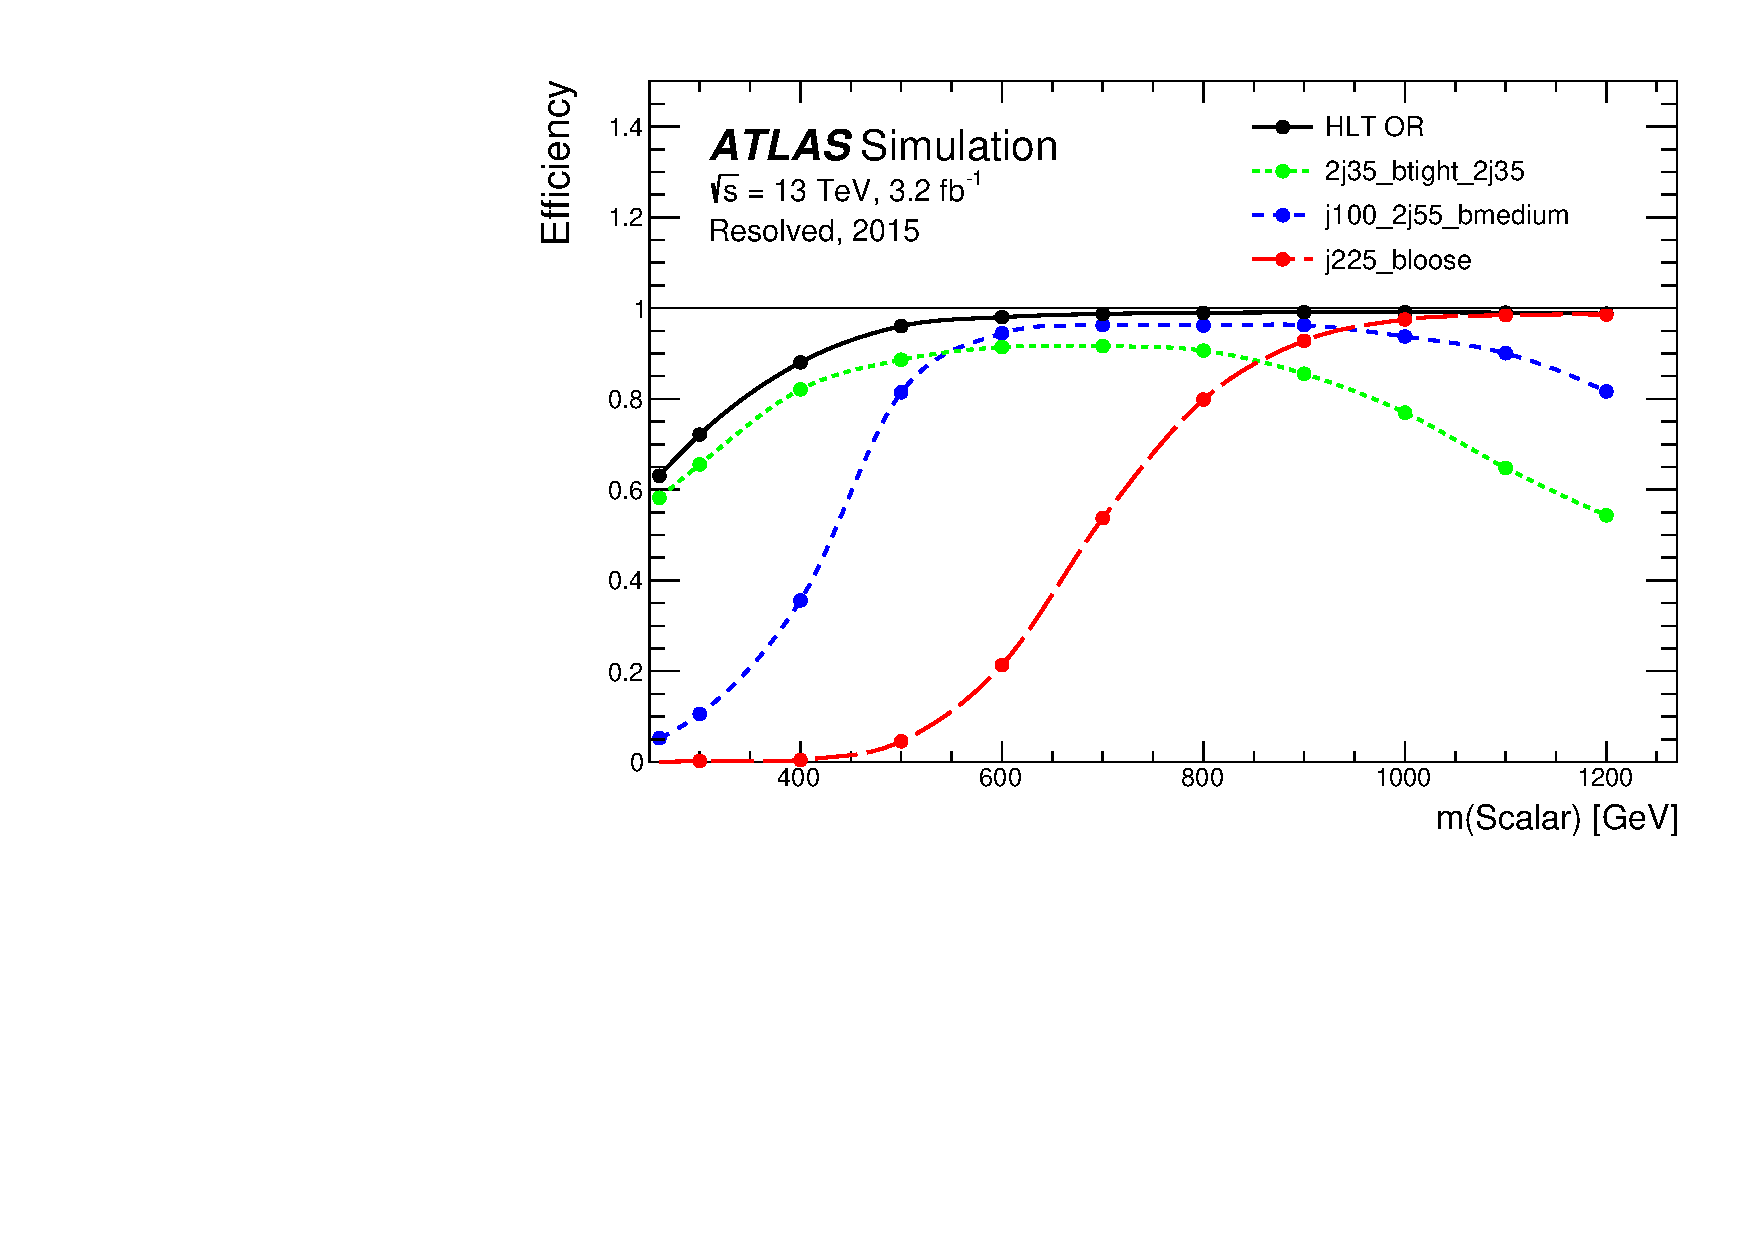
\includegraphics[width=\textwidth,angle=-90]{figures/resolved/extra_plots/trigEff_2015_NWS_passSignal_HLT}
        \caption{2015}
        \label{fig:data_restrig_2015}
    \end{subfigure}
    \quad \quad \quad \quad \quad \quad
    \begin{subfigure}[b]{0.28\textwidth}
        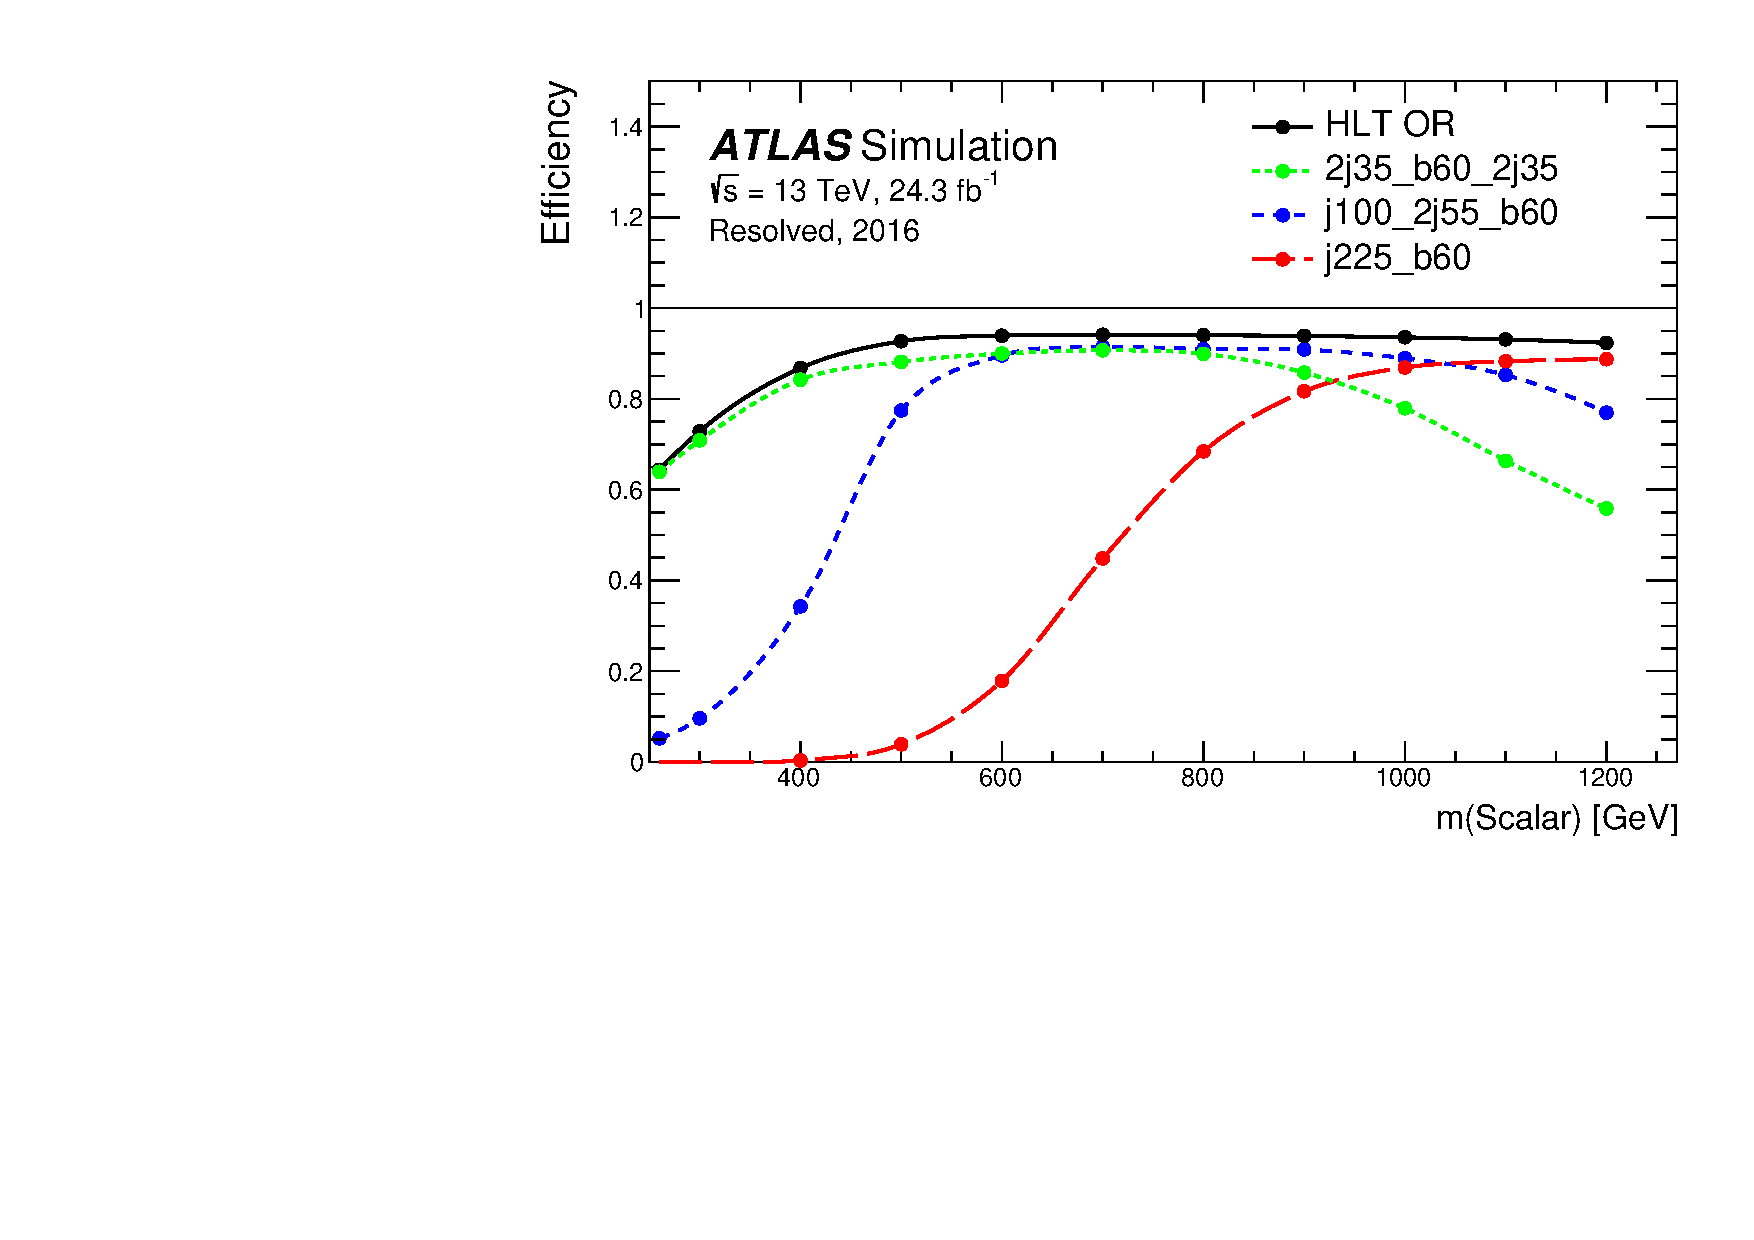
\includegraphics[width=\textwidth,angle=-90]{figures/resolved/extra_plots/trigEff_2016_NWS_passSignal_HLT}
        \caption{2016}
        \label{fig:data_restrig_2015}
    \end{subfigure}
\caption{Trigger efficiencies following the full resolved analysis selection as a function of the resonance signal mass. The efficiencies of the triggers used in 2015 and 2016 are shown. In both graphs, the green line shows the efficiency of the ``2b4j'' trigger; the blue line represents the ``2b3j'' trigger; the red line represents the ``1b1j'' trigger. The 2016 triggers are less efficient due to a bug in the online primary vertex reconstruction.}
\label{fig:data_restrig}
\end{figure}

\paragraph{}
During 2016 data-taking, a fraction of the data was affected by a bug.
The movement of the beam spot was not accounted for in the on-line vertex reconstruction.
This reduced the efficiency of the algorithms used to identify $b$-jets.
That fraction of data is not used and this reduces the integrated luminosity of the 2016 dataset for the resolved analysis to $24.3$ \ifb.

\paragraph{}
In the boosted analysis, events were selected from the 2015 dataset using a trigger that required a single anti-$k_t$ jet with radius parameter $R=1.0$ and with \pt~$>360$~\GeV. In 2016, a similar trigger was used but with a higher threshold of \pt~$>420$~\GeV. The efficiency of these triggers is 100\% for simulated signals passing the jet requirements as described later, so the 2015 and 2016 datasets were combined into one dataset. 

\paragraph{}
The data is further skimmed into the Derived Analysis Object Data (DAOD). The ATLAS off-line software 20.7.8.7 derivation cache is used, with version $p$-tags \textit{p2950}. The boosted slimming keeps events with at least two large-\R jets with \pt~$>200$ \GeV. The final input data file has name format: $dataYR\_13TeV.periodPR.physics\_Main.PhysCont.DAOD\_EXOT8.grpYR\_v01\_p2950$, where YR is $15$ and PR is DEFGHJ for 2015 data, and YR is $16$ and PR is ABCDEFGIKL for 2016 data.


\section{MC}
\paragraph{}
All Monte Carlo (MC) samples used in this analysis are produced with full simulation.
For all simulated samples, charm-hadron and bottom-hadron decays were handled by {\textsc{EvtGen}} 1.2.0~\cite{EvtGen}. 
To simulate the impact of multiple low momentum $pp$ interactions that occur within the same or nearby bunch crossings, minimum-bias events generated with \pythia~8~\cite{Sjostrand:2006za} using the A2 set of tuned parameters~\cite{MC12AU2} were overlaid on the hard-scatter event.
This pile-up effect is simulated with a $\mu$ of $25$.
Although this is different from the pile-up level in data, it has little effect on the analysis and the pile-up reweighting is not adopted.
%https://twiki.cern.ch/twiki/bin/view/AtlasProtected/AtlasProductionGroupMC15c#Pileup_for_samples_with_small_nu
The detector response was simulated with GEANT~4~\cite{Agostinelli:2002hh, Aad:2010ah} and the events were processed with the same reconstruction software as that used for the data.  
Simulated data samples from the ATLAS MC15c campaign are be used, corresponding to $p$-tags \textit{p2952-p2949}.

\section{Signal}
\paragraph{}
In all signal samples, the mass of the Higgs boson ($m_H$) was set to 125~\GeV. 
The signal MC contains truth information, such as the two Higgs and the b quark four-momenta before detector interactions. 
This enables a $\Delta R$ truth matching between the reconstructed objects and the Higgs.

\paragraph{}
SM non-resonant production of Higgs boson pairs via the gluon--gluon fusion process was simulated at NLO with \texttt{MG5\_aMC@NLO}, using form factors for the top-quark loop from HPAIR~\cite{PhysRevD.58.115012, Plehn199646}. 
The simulated events are reweighted to reproduce the \mhh~ spectrum obtained~\cite{Borowka:2016ehy, Borowka:2016ypz}. 
This spectrum is calculated at NLO in QCD while fully accounting for the top-quark mass. 
Interference effects between di-Higgs resonant production and SM non-resonant di-Higgs production are not included in the simulated samples. 
%The cross section times branching ratio to the \fourb\ final state is $11.3^{+0.9}_{-1.0}$~fb~{\cite{Borowka:2016ehy}.
%The uncertainty includes the effects due to renormalization and factorization scales, PDF set, $\alpha_{\mathrm{S}}$, and the \hbb\ branching ratio. 

\paragraph{}
Signal \Gtohhb\ events were generated at leading order (LO) with \texttt{MG5\_aMC@NLO}~2.2.2~\cite{MGaMCatNLO} interfaced with \pythia~8.186 for parton-showering, hadronization and underlying-event simulation. 
The NNPDF2.3 LO parton distribution function (PDF) set~\cite{Ball:2012cx} was used for both \texttt{MG5\_aMC@NLO} and \pythia. 
The A14 set of tuned underlying-event parameters was used. 
These signal samples were generated with $\kMPl = 1$ or $2$.
Relative to the resonance mass, widths of the graviton signals range from 3\% (at low mass) to 13\% (at the highest mass) for $\kMPl=1$, and $6\%$ to $25\%$ for $\kMPl=2$.
The graviton samples were normalized using fixed cross sections~\cite{carvalho}.

\paragraph{}
Signal 2HDM Scalar \tohhb\ events were generated at LO in QCD with \texttt{MG5\_aMC@NLO}~2.2.3 interfaced with \textsc{Herwig++}~\cite{Bahr:2008pv} for parton-showering, hadronization and simulation of the underlying event. CT10~\cite{Lai:2010vv} PDF sets were used for \texttt{MG5\_aMC@NLO} and CTEQ6L1~\cite{cteq6l1} for \textsc{Herwig++}.
The UE-EE-5-CTEQ6L1 set of tuned underlying-event parameters \cite{Seymour:2013qka} was used. 
The scalar signals were generated with a width of $1$~\GeV, which represent generic narrow-width scalar signals. 
Because the width and branching ratios depend on 2HDM parameters, each mass point generated with this fixed width corresponds to a different point in the 2HDM parameter phase space.
%No specific model was considered for computing the scalar signal cross sections.
%For the evaluation of theoretical uncertainties in the signal modeling, samples were produced with variations of the factorization and renormalization scales, PDF sets (following the prescription from Ref.~\cite{pdfs}) and shower generator. For the latter, scalar (spin-2) samples were produced that are interfaced to \PYTHIA~8.186 rather than \textsc{Herwig++} (and vice versa).

\paragraph{}
Resonant signal samples for the scalar and $\kMPl=1$ models were produced in $10$~\GeV\ steps between $260$ and $300$~\GeV, in $100$~\GeV\ steps up to $1600$~\GeV, in $200$~\GeV\ steps up to $2000$~\GeV, and in $250$~\GeV\ steps up to $3000$~\GeV. Signal samples for the $\kMPl=2$ model were produced with the same spacings but omitting the masses of $270$~\GeV, $290$~\GeV\ and $2750$~\GeV\ due to the larger generated width. Unless specified, the MC signal sample used as benchmark is $\kMPl=1$ \Grav, due to its width is medium among the three signal models.

\subsection{Backgrounds}
\paragraph{}
A very small fraction of the background arises from $Z$ + jets events. The $Z$+jets sample was generated using \pythia~8.186 with the NNPDF2.3 LO PDF set.

\paragraph{}
The \ttbar\ background is modeled using large all-hadronic and non-all-hadronic samples that have both been generated with \powhegbox\ v1~\cite{Alioli:2010xd} using the CT10 PDF set. 
The parton shower, hadronization, and the underlying event were simulated using \pythia~6.428 with the CTEQ6L1 PDF set and the corresponding Perugia 2012 set of tuned underlying-event parameters~\cite{Skands:2010ak}.
The $t$-quark mass in both samples is set to $172.5$ \GeV~.
Higher-order corrections to the \ttbar\ cross section were computed with Top++~2.0~\cite{Czakon:20142930}. These incorporate NNLO corrections in QCD, including re-summation of NNLL soft gluon terms.
The \ttbar\ MC samples are normalized to the NNLO+NLL predicted inclusive \ttbar\ cross-section of
$1821.87$ pb multiplied by the all-hadronic branching ratio of $0.457$ and non-all-hadronic of $0.543$.

\paragraph{}
In order to minimize statistical fluctuations across the dijet invariant mass spectrum, especially for large values of $m_{tt}$, additional \ttbar~ samples are generated in slices of \ttbar~ invariant mass. The cross-section of the \ttbar~ process is normalized to NNLO+NNLL in QCD, as calculated by \textsc{Top++} 2.0. Overlap with the inclusive \ttbar~ samples is removed by a fixed cut on the truth value of $m_{tt}$ at $1100$ \GeV.

\paragraph{}
A \pythia~ dijet sample is used to understand the multi-jet background and characteristics of the event selection. This MC sample is generated without a heavy flavor filter, hence is limited by the total generated number of events, given the high background rejection factors of the analysis selection.











